\chapter{Background Research \& Notation}
\label{chapter2}
Within this chapter, we begin by introducing the formal method for representing sequential decision making problems. We then proceed to formally introduce Planning and discuss some algorithms of interest. We finish by formally introducing Reinforcement Learning, the various encapsulations of RL and providing a short survey of exploration methods in RL; this survey is the main bulk of our literature review.
\section{Markov Decision Processes}
The Markov Property states that the future is conditionally independent of the past given the present. A sequential decision-making problem that satisfies the Markov Property is known as a Markov Decision Problem, and can be modelled by a Markov Decision Process (MDP) \cite{10.5555/528623}. Where an agent is able to fully observe its state, the problem can be modelled as an MDP. Conversely, where an agent can only partially observe its state, the problem can be modelled by a Partially Observable Markov Decision Process (POMDP).
Consider an agent playing a perfect information game, such as Chess or Go, the agent (and its opponent) are able to fully observe the state of the game with ease. However, a robot navigating through a maze may not be able to observe its exact state due to uncertainty in its sensors.
Furthermore, an MDP can be stationary or non-stationary which refer to whether its dynamics stay the same, or change temporally.
An MDP that contains absorbing states, that is any state that upon entering the task terminates, then is said to be episodic.
\\Within this work we assume that the agent is fully able to observe its state, the environment is stationary and can be discretised in some way and tasks are episodic.
Hence we consider \textbf{stationary}, \textbf{finite}, \textbf{undiscounted} MDPs.
Thus, an MDP is a 4-tuple, $\text{MDP} = (S,A,T,R)$ where:
\begin{itemize}
    \item $S$ is a finite set of states.
    \item $A$ is a finite set of actions.
    \item $T : S \times A \times S \rightarrow [0,1]$ is the transition function, which determines the probability of transitioning from a state $s \in S$ to $s' \in S$ with an action $a \in A$.
    \item $R:S \times A \times S \rightarrow \mathbb{R}$ is the reward function, which determines the reward signal, $r \in \mathbb{R}$ received by the agent from transitioning from a state $s \in S$ to $s' \in S$ with the action $a \in A$. This reward is extrinsic to the agent; it comes from the environment.
\end{itemize}
\begin{defn}
\label{defn:determinism}
An MDP is said to be deterministic if $\forall s,s' \in S, \forall a \in A$, $T(s,a,'s) \in \{0,1\}$.
\end{defn}
\begin{defn}
\label{defn:stochastic}
An MDP is said to be stochastic if it is not deterministic
\end{defn}
\subsection{Policies, Value and Quality}
A policy, denoted by $\pi$, is a mapping of states to actions that describes a behaviour within an MDP. The desired behaviour within an MDP is to maximise the cumulative reward, this is known as the optimal policy and denoted $\pi^*$. The cumulative reward is given by:
\begin{equation}
\label{eqn:return}
G_t = \sum_{k=t+1}^TR_{k}
\end{equation}
which represents the cumulative reward received from time $t$ to some finite time $T$.
A Value Function, or state-value function, denoted $V^\pi(s)$, measures the expected cumulative reward that can be received starting in each state $s \in S$ and following a policy $\pi$:
\begin{equation}
\label{eqn:vs}
    V^\pi(s) = \mathbb{E}^\pi\Bigg[G_t | s_t = s\Bigg] = \mathbb{E}^\pi\ \Bigg[\sum_{k=t+1}^TR_{k} | s_t = s \Bigg]
\end{equation}
Where $\mathbb{E}$ represents the expected value that the agent follows $\pi$, $t$ is an arbitrary time step and $T$ is a finite time horizon.
The optimal Value Function, $V^*$, is the one that is maximum for every $s \in S$ and is given by:
\begin{equation}
\label{eqn:vsm}
     V^*(s) = \max_\pi V^\pi(s) 
\end{equation}
This can also be represented in a recursive form, known as the Bellman Optimality equation for $V$:
\begin{equation}
\label{eqn:vsB}
V^*(s) = \max_a\sum_{s'}T(s,a,s')[R(s,a,s')+V^*(s')]
\end{equation}
Similarly, a Q-Function, or action-value function, denoted $Q^\pi(s,a)$, measures the expected cumulative reward that can be received starting in each state $s \in S$, taking an action $a \in A$ and thereafter following a policy $\pi$:
\begin{equation}
\label{eqn:qsa}
Q^\pi(s,a) = \mathbb{E}^\pi\Bigg[G_t | s_t = s,a_t = a\Bigg] = \mathbb{E}^\pi\Bigg[\sum_{k=t+1}^TR_{k}|s_t=s, a_t = a\Bigg]
\end{equation}
Where $\mathbb{E}$ represents the expected value that the agent follows $\pi$, $t$ is an arbitrary time step and $T$ is a finite time horizon.
The optimal Q-Function, $Q^*$, is the one that is maximum for every $s,a \in S \times A$ and is given by:
\begin{equation}
\label{eqn:qso}
Q^*(s,a) = \max_\pi Q_\pi(s,a)
\end{equation}
Similarly to the Value Function, this can also be represented in a recursive form, known as the Bellman Optimality equation for $Q$:
\begin{equation}
\label{eqn:qsB}
Q^*(s,a) = \sum_{s'}T(s,a,s')[R(s,a,s')+\max_{a'}Q^*(s',a')]
\end{equation}
An interesting observation is that $\pi^*$ can be derived from both $V^*$ and $Q^*$. In the case of $V^*$, $\pi^*$ can be derived by determining at each state, which actions yield the next state with the maximum value. In the case of $Q^*$, $\pi^*$ can be derived by simply taking the action with the highest Q-value at each state \cite{Sutton1998}.

\section{Planning}
Planning involves reasoning on a model of an environment, in order to produce a sequence of successive actions that will achieve a specified goal whilst satisfying some constraints or achieving some objectives, such as minimising cost \cite{GhallabNauTraverso04, Lav06, DBLP:books/aw/RN2020}.
\\In the context of MDPs, the goal is to maximise cumulative reward. Formally, let $s_t \in S$ be some start state at a discrete time, $t$. The goal of the planner is to produce a sequence of actions, $P=(a_t, a_{t+1},...,a_{t+n})$, such that $\pi^*(s_t) = P(t)$, for all $t$.
% \\Formally, the goal of Planning is given an MDP, $M$, start and goal states, $s$ and $g$, to produce a sequence of actions, $P=(a_0, a_1,...,a_n)$, such that executing $P$ would result in transitioning from the start state to the goal state.
\\Planning has been a widely studied topic in AI for many years and as such there exist many planning methods and algorithms. While the use of Planning is central to this work, particular planning methods and algorithms are not; therefore, we only consider heuristic search methods and planning by Dynamic Programming.
\subsection{Heuristic Search}
Heuristic search (or informed search) \cite{EdelkampSchroedl11} is a class of search algorithms that use problem specific knowledge in the form of heuristics to guide the search. A heuristic, denoted $h(s)$, is a function that estimates the cost of transitioning from the current state, $s$, to the goal state. We consider best-first search algorithms, which aim at expanding states that appear best according to an evaluation function, denoted $f(s)$. 

\subsubsection{A* Search}
\label{sec:astar}
A* Search (or just A*) \cite{4082128} is a heuristic search algorithm that is a form of best-first search. A cost function, $g(s)$, is introduced, which indicates the cost to get from the start state to a state $s$. The main idea is that the evaluation function can be a combination of the cost to get to the state being evaluated, $g(s)$, and the estimated cost to get from the state being evaluated to the goal state, thus:
\begin{equation}
\label{eqn:astarr}
f(s) = g(s) + h(s)
\end{equation}
The evaluation function indicates the estimated cost of the minimum cost solution that passes through $s$ \cite{DBLP:books/aw/RN2020}. A* works by guiding the search to expand states with the lowest value for $f(s)$ first, in order to determine a sequence of states which is the path (or in our case, the plan). A* is a complete algorithm; it will always find a solution if one exists. However, the optimality of A* depends on the choice of the heuristic: the heuristic must be admissible, which means that it must never overestimate the cost of getting from the current state to the goal state; in this sense, the heuristic must always be optimistic.

\subsection{Dynamic Programming}
Dynamic Programming (DP) \cite{Bellman:1957, DBLP:books/lib/Bertsekas05} refers to a collection of methods that can be used to solve MDPs, by computing the optimal policy with respect to them. The two main algorithms that we consider are Policy Iteration and Value Iteration; both of which are forms of Generalised Policy Iteration (GPI). GPI refers to any process that involves Policy Evaluation and Policy Improvement acting with each other. As it happens, most DP and RL methods are forms of GPI \cite{Sutton1998}.

\subsubsection{Policy Evaluation and Improvement}
Given a policy, $\pi$, it can be evaluated by computing its Value Function, $V^\pi$:
\begin{equation}
\label{eqn:policyeval}
V^\pi = \sum_a \pi(a|s)\sum_{s'}T(s,a,s')[R(s,a,s') + V^\pi(s')]
\end{equation}
Policy Improvement is the process of generating an improved policy from a suboptimal policy \cite{DBLP:books/lib/Bertsekas05}. A policy $\pi$ could be improved by contemplating taking an action $a \in A$ in a state $s \in S$, such that $\pi(s) \neq a$ and then continue following $\pi$ thereafter. We can evaluate this change by computing the Q-function for $s,a$:
\begin{equation}
\label{eqn:qval}
Q^\pi(s,a) = \sum_{s'}T(s,a,s')[R(s,a,s') + V^\pi(s')]
\end{equation}
Then comparing $Q^\pi(s,a)$ with $V^\pi(s)$. If $Q^\pi(s,a) > V(s)$, then the policy is update and improved as such: $\pi(s) = a$.
\subsubsection{Policy Iteration}
Policy Iteration (PI) \cite{Bellman:1957, howard:dp} is a method for computing the optimal policy of an MDP. Assuming an arbitrary initial policy, $\pi$, at each step $\pi$ is evaluated, yielding a Value Function $V^\pi$ (or a Q-Function $Q^\pi$). The policy is then updated greedily with respect to $V^\pi$ (or $Q^\pi$). This iterative process leads to monotonic improvements to $\pi$.
\subsubsection{Value Iteration}
Value Iteration (VI) \cite{Bellman:1957} is a method for computing the optimal estimate for the Value or Q-Function of an MDP. As the estimate approaches optimality, the policy that is greedy with respect to the Value or Q-Function also approaches optimality \cite{series/synthesis/2010Szepesvari}.
In the context of Value Functions, assuming an arbitrary initial estimate, $V$, at each step $V$ is updated as such:
\begin{equation}
\label{eqn:vupdate}
V(s) = \max_a\sum_{s'}T(s, a, s')[R(s, a, s')+V(s')]
\end{equation}
for all $s \in S$. This update originates from the Bellman optimality equation for $V$, Equation \ref{eqn:vsB}.
For Q-Functions, assuming an arbitrary initial estimate, $Q$, at each step $Q$ is updated as such:
\begin{equation}
\label{eqn:qupdate}
Q(s,a) = \sum_{s'}T(s,a,s')[R(s,a,s') + \max_{a'}Q(s',a')]
\end{equation}
for all $s \in S$, $a \in A$. This update originates from the Bellman optimality equation for $Q$, Equation \ref{eqn:qsB}.

\section{Reinforcement Learning}
Within an RL setting, formalised by an MDP, an agent learns how to behave in an environment by interacting with it through actions, at discrete, sequential, time steps, and observing the affects through its new state and a scalar reward signal, as seen in Figure \ref{fig:rl}. The reward signal may be delayed, meaning that the consequences of actions may not be known until long after they are taken \cite{barto1990learning}. This gives rise to the (temporal) credit assignment problem \cite{Minsky:1961:ire}, the problem of determining which actions led to an outcome and assigning credit among them; it's often the case that a sequence of actions led to an outcome, rather than a single action. The ultimate goal of the agent is to learn a policy, $\pi^*$, that maximises the expected cumulative long-term reward \cite{Sutton1998}; as we outlined in Chapter \ref{chapter1}, exploration, exploitation and the trade-off between the two, are key to this. The two main instantiations of RL are model-free and model-based, each of which we will delve deeper into within this section.
\begin{figure}[h!]
    \centering
    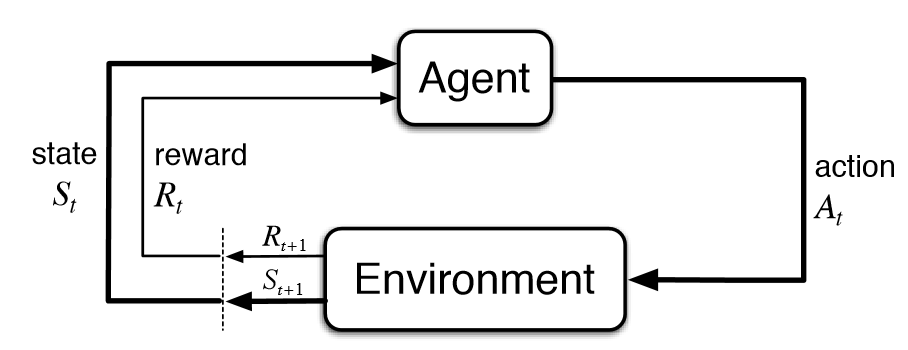
\includegraphics[max size={325pt}{325pt}]{report/assets/rl.png}
    \caption{The RL Loop \cite{Sutton1998}}
    \label{fig:rl}
\end{figure}

\subsection{Model-free RL}
Model-free (or direct) is where the agent learns a policy directly from experience gained by interacting with the environment; it is purely trial-and-error. Model-free learning tends to be quite flexible to varying problems, since no assumptions are made about the environment's dynamics. Furthermore, since the environment's dynamics do not need to be stored, learned or considered, model-free learning is scalable and does not suffer from the \textit{curse of dimensionality} (in the non-tabular cases) and can be computationally efficient, as there is generally no lookahead deliberation process involved. However, model-free learning can be sample-inefficient; the agent may need to take many actions before discovering the optimal policy. Moreover, in real-world domains, model-free learning may not even be feasible, due to the cost of experience. The most common model-free approach is Temporal Difference Learning.

\subsubsection{Temporal Difference Learning}
Temporal Difference (TD) Learning \cite{10.5555/911176, 5392560, 5391906} aims at solving the problem of temporal credit assignment by combining ideas from Monte Carlo methods, which learn directly from experience in the environment, and Dynamic Programming methods, which bootstrap estimates from other previously learned estimates; it is a form of GPI \cite{Sutton1998}.
% It is a form of Generalised Policy Iteration, in that it aims to produce an optimal estimate of the Value Function, $V_\pi^*$, starting from an initial estimate, $V_\pi$, for a given policy, $\pi$,\cite{Sutton1998}.
\\The core idea of TD Learning is to update the estimate of the Value Function, $V_\pi$, whenever there is a difference between temporally successive predictions. This difference is known as the TD error. The updated estimate is bootstrapped from the previous estimate, meaning that TD learning essentially learns a prediction from another prediction.
\\The simplest TD Learning algorithm is TD(0), which updates it's estimates as such:
\begin{equation}
\label{eqn:td0update}
V(s_t) = V(s_t) + \alpha[r_{t+1} + V(s_{t+1}) - V(s_t)]
\end{equation}
The TD target is the current prediction of the expected cumulative reward: $r_{t+1} + V(s_{t+1})$, the TD error is $r_{t+1} + V(s_{t+1}) - V(s_t)$ and $0 \le \alpha \le 1$ is the learning rate, which is used to control how much weight is given to the TD error when updating the estimate \cite{Sutton:1988}.
\\TD Learning can also be extended to learn a Q-Function, which stores the value of state-action pairs rather than the value of states. For each state-action pair, it stores an estimate of the expected cumulative reward starting in that state and taking an action, and following a fixed policy. This can be done using Q-Learning and SARSA.

\paragraph*{Q-Learning} \cite{Watkins:1989, journals/ml/WatkinsD92} is an off-policy TD Learning method that learns a Q-function. It is off-policy, as the update rule assumes a greedy policy - this means that the value of the optimal policy is learned independently of the agent's actions following the current policy. Q-values are iteratively updated using the Bellman equation, the update rule is as follows:
\begin{equation}
\label{eqn:qlearningupdate}
Q(s_t,a_t) = Q(s_t,a_t) + \alpha[r_{t+1} + \max_aQ(s_{t+1}, a) -Q(s_t,a_t)]
\end{equation}
\paragraph*{SARSA} (State Action Reward State Action) \cite{rummery:cuedtr94} is an on-policy TD Learning method that learns a Q-function. It is on-policy, as the update rule assumes that the current policy continues being followed - this means that the value of the current policy being followed is learned. Q-values are iteratively updated using the Bellman equation, the update rule is as follows:
\begin{equation}
\label{eqn:sarsaupdate}
Q(s_t, a_t) = Q(s_t, a_t) + \alpha[r_{t+1} + Q(s_{t+1}, a_{t+1})-Q(s_t, a_t)]
\end{equation}

\subsection{Model-Based Learning}
Model-based (or indirect) RL is where an agent uses a known or learned model of the environments dynamics (in the form of an MDP) in order to learn an optimal policy. The agent may learn the model and policy at the same time, as in the Dyna family \cite{Sutton:1990, 10.1145/122344.122377} or learn a policy by planning over a known model, as in AlphaZero \cite{DBLP:journals/corr/abs-1712-01815} or learn a policy by planning over a learned model, as in MuZero \cite{DBLP:journals/corr/abs-1911-08265}. Model-based RL offers improved real-world sample efficiency, potential for directed, informed exploration and better asymptotic performance, the prospect of transfer learning, safer learning and explainability \cite{MAL-086}. These benefits come at a computational cost, typically in planning; however we take the stance that this added computational cost is certainly worth it, particularly for the benefit of reducing learning costs. 
Since it's not always the case that a model is known as a priori, and even if it is it might be inaccurate, model-learning is a key component of model-based RL.

\subsubsection{Model Learning}
Model Learning can be difficult due to uncertainty caused by limited data and stochasticity. Uncertainty can be overcome through sufficient exploration; sampling a transition multiple times can give a better estimate of its probability distribution.
\\Model learning can be viewed as a supervised learning problem \cite{JORDAN1992307}. In discrete environments, exact models of the environment's dynamics can be learned in the form of a \textit{tabular maximum likelihood model} \cite{10.1145/122344.122377} which  maintains a table with an entry for every possible transition.
In the stochastic case, for each transition the table will store:
\begin{equation}
\label{eqn:tmlmupdate}
T(s, a, s') = \frac{n(s, a, s')}{\sum_{s'}n(s,a,s')}
\end{equation}
Where $n : S \times A \times S \rightarrow \mathbb{Z}$ represents the number of times a transition has been observed. This also works for the deterministic case, which will result in all transitions mapping to either 0 or 1; but this leads to unnecessary computations; it's better to manually update $T$ if the domain is known to be deterministic.
A key drawback to this approach is the lack of scalability to large state spaces.
\\In continuous domains an exact model cannot be learned, due to the infinite number of states (and potentially actions). An approximate model can be learned by using state aggregation (which discretises the state space) and a tabular maximum likelihood model \cite{Kuvayev1996ModelBasedRL}.
\\In continuous domains its impossible to learn an exact tabular model, and it may also be infeasible for discrete domains with large state spaces, therefore an approximate model must be learned; most commonly this is done through Function Approximation methods, such as Linear Regression \cite{DBLP:journals/corr/abs-1206-3285, NIPS2007_b7bb35b9} and Gaussian Processes \cite{10.5555/3104482.3104541}.

\section{Exploration Methods in Reinforcement Learning}
Within this section, we will provide a brief survey of exploration methods in RL. Whilst Thrun distinguished between undirected and directed exploration \cite{Thrun-1992-15850}, and Amin et al. distinguished between reward-free and reward-based exploration \cite{DBLP:journals/corr/abs-2109-00157}, there is no definitive taxonomy of exploration methods; as such, we will use our own categories, which distinguishes between model-free, model-based and hybrid approaches.
\subsection{Model-Free Methods}
Model-free exploration methods are characterised by the fact that they do not use, or learn, a model to aid exploration. This means that they can be robust to varying domains, where designing or learning a model could prove difficult. However, they must rely on other methods to drive exploration, which tend to be grounded in randomness.
\\Purely random exploration comes in the form of a Random Walk, or unguided random search \cite{anderson86}, which arises from randomly sampling actions with uniform probability. Exploration occurs naturally when the agent moves away from the goal, rather than closer to it. This is perhaps the most naive exploration method, since it is entirely random, and thus it is very inefficient and rarely used in practice.
\\ Boltzmann exploration samples an action according to the Boltzmann distribution:
\begin{equation}
\label{eqn:boltzmann}
\pi(a|s) = \frac{e^{Q(s,a)/\tau}}{\sum_{a' \in A}e^{Q(s,a')/\tau}}
\end{equation}
Where the temperature, $0 \le \tau \le 1$, is a hyperparameter that determines how frequently random actions are chosen; as $\tau$ approaches 0, the policy approaches greediness \cite{Thrun-1992-15850, DBLP:journals/corr/abs-2109-00157}. When there are large differences between Q-values, little exploration occurs, however when Q-values are close to each other, considerable exploration occurs. This means that Boltzmann exploration has a particular reliance on the initialisation of the Q-values, and the early exploration \cite{wiering}. Moreover, Boltzmann exploration does not consider uncertainty in Q-values \cite{DBLP:journals/corr/Cesa-BianchiGLN17}, which can lead to actions being chosen which appear to be promising, but in reality are not, due to epistemic uncertainty. 
% Various modifications have been suggested to Boltzmann exploration to overcome its problems, such as using learning-rate schedules to attenuate the temperature \cite{singh00} and per-action learning rates \cite{DBLP:journals/corr/Cesa-BianchiGLN17}.
\\$\epsilon$-greedy \cite{Watkins:1989, conf/nips/Sutton95} uses a hyperparameter, $0 \le \epsilon \le 1$ to explicitly balance between exploration and exploitation. With probability $\epsilon$ the agent explores by taking a random action, which is sampled with uniform probability, with probability $1-\epsilon$ the agent exploits by taking the best action, which is selected greedily with respect to the current policy. Uniformly choosing actions means that actions which are known to be sub optimal can be continually evaluated long after they are realised to be so.
\\Pure random exploration is very inefficient, and certainly not a practical exploration method. Boltzmann exploration and $\epsilon$-greedy offer better exploration strategies than pure randomness, but they are not without their faults. Moreover, model-free methods in general tend to lack temporal persistence which can lead to indecisiveness during exploration, for instance moving back and forth between two states, leading to inefficient exploration. Extensions have been proposed to Boltzmann exploration and $\epsilon$-greedy that overcome some of their respective issues, such as Boltzmann-Gumbel exploration \cite{DBLP:journals/corr/Cesa-BianchiGLN17} and $\epsilon z$-greedy \cite{dabney2021temporallyextended}, although the standard methods seem to favoured in practice.
%  h e Boltzmann rule causes a lot of exploration in states where Q-values for different
% actions are almost equal, and little exploration in states where Q-values are very different.
% This is helpful for risk minimization purposes (Heger, 1994), for which we may prefer not
% to explore actions which look significantly worse t h a n others. However, initially learned Q-
% estimates can be incorrect due to noise, so some exploration is still needed in case of large
% differences in Q-values. Using an annealing schedule for the t e m p e r a t u r e should get around
% this problem, b u t finding a good annealing schedule can be quite difficult and is reward
% function dependent.2 Furthermore, since the t e m p e r a t u r e is a global variable, it may happen
% t h a t some state is not visited for a long time, after which the amount of exploration in
% this state is very small. Although this last problem could be solved using local t e m p e r a t u r e
% variables, it is still a problem t h a t the agent may concentrate on different trajectories which
% it already knows well.


% \\ Pure random exploration is extremely inefficient, and will likely not succeed in complex domains. Boltzmann exploration and $\epsilon$-greedy offer a stronger solution than pure randomness, but they still have their respective limitations, which can lead to getting stuck in a local optima.

% While model-free exploration methods can be robust and applicable to a wide range of domains, they also come with some weaknesses. Random exploration can be highly inefficient and often fails to achieve the exploration goals within reasonable time constraints. Boltzmann exploration and ε-greedy methods are more efficient than random exploration, but they still have limitations. Boltzmann exploration may not work well in environments where the optimal action is much better than the suboptimal ones, as it may lead to the agent choosing suboptimal actions too often. Similarly, ε-greedy methods may not be effective in environments where there are many equally good actions, as the agent may get stuck in a suboptimal action instead of exploring all possible options. Therefore, while these methods have their advantages, it is important to consider their limitations and choose the exploration strategy that is best suited to the particular domain and task at hand.

% Whilst Boltzmann Exploration and $\epsilon$-greedy are simple exploration strategies that are very commonly used in practice, they suffer from a variety of issues. Firstly, there is no temporal persistence. There is als
% \\ Boltzmann Exploration and $\epsilon$-greedy are very commonly use exploration methods in practice.
\subsection{Model-Based Methods}
Conversely to model-free exploration methods, model-based exploration methods are those that use, or learn, a model that is used to drive exploration.
\subsubsection{Optimistic}
Optimistic exploration methods are based on the \textit{optimism in the face of uncertainty} (OFU) principle \cite{DBLP:journals/corr/cs-AI-9605103}.
\\Explicit, Explore or Exploit ($E^3$)  \cite{Kearns+Singh:2002} maintains a partial model of the environment through collecting statistics, akin to the \textit{tabular maximum likelihood} approach. A distinguishment is made between \textit{known} and \textit{unknown} states; a state is \textit{known} after it has been visited an arbitrary number of times, thus its learned dynamics must be close to the true dynamics. If the current state is \textit{unknown}, then \textit{balanced wandering} takes place, and the agent explores by selecting the action that has been taken the least number of times from that state. If the current state is \textit{known}, then an exploitation policy and an exploration policy are computed. One of these policies is chosen and followed for a finite time horizon; exploitation is chosen if the policy will induce large cumulative reward, exploration is chosen otherwise.
\\ R-MAX \cite{10.1162/153244303765208377} is an extension and generalisation of $E^3$. It begins with an optimistic initial model such that every transition leads to some imaginary state, \textit{The Garden of Eden State}, that returns the maximal reward, denoted $R_{max}$. R-MAX uses the same concept of \textit{known} and \textit{unknown} states as in $E^3$; after a state becomes known, then the model is updated with the collected statistics regarding that state. The agent always follows the optimal policy according to the model. R-MAX removes the need for explicit contemplation between exploring and exploiting as in $E^3$; exploration and exploitation occur naturally.
\\ Optimistic Intial Model (OIM) \cite{10.1145/1390156.1390288} begins with an optimistic model, the same as R-MAX. The model is updated through observations similarly to $E^3$. The agent maintains two Q-functions; one for the real extrinsic rewards, and one for intrinsic exploration rewards. Whilst exploring, the agent acts optimally with respect to the combination of the two Q-functions; thus the latter Q function can be seen as an exploration bonus. During this, the agent will either act near-optimally, or will gain new information it can utilise. After exploration is terminated, perhaps after a certain number of time steps, the agent acts optimally with respect to the Q-function based on extrinsic rewards.
% \\ UCRL \cite{NIPS2006_c1b70d96} \textbf{UCRL explanation}
% \textbf{Conclusions about optimistic approaches}
\\ $E^3$, R-MAX and OIM are provably able to achieve near-optimal performance in polynomial time in discrete environments, however they don't tend to be very efficient in practice. R-MAX and OIM in particular show that optimism is definitely a useful heuristic, but they are very optimistic in perhaps an unrealistic way; an interesting question to ask is whether this unrealistic level of optimism necessary, and if a \textit{reasonable} level of optimism is just as useful. These methods also assume that the model will eventually become correct, which may not be the case in complex tasks, and in the worst case will learn the entire model, leading to wasted exploratory steps.
\subsubsection{Intrinsically Motivated}
Model-Based Active Exploration (MAX) \cite{DBLP:journals/corr/abs-1810-12162} is purely an exploration framework, which pure exploitation could follow from. An ensemble of dynamics models is maintained and trained on new observations. At each time step a model is sampled from the ensemble, and a one-step policy is derived from the model such that it maximises the intrinsic reward function, which indicates novel states using expected information gain, based on the Jensen-Shannon Divergence.
\\Plan2Explore \cite{plan2explore} separates learning in to two separate phases. During the first phase, the agent learns a global model of the environment, in the form of a latent dynamics model, whilst maintaining and training an ensemble of models on new observations. To explore, the agent trains an exploration policy in the world model that aims to seek out novel states; novelty is defined by estimating latent disagreement in the ensemble of models with the global model. In the second phase, the agent adapts to downstream tasks by using the extrinsic reward signals.
\\ MAX and Plan2Explore both perform task-agnostic exploration, which they claim means they can generalise to downstream tasks easily. However, only Plan2Explore was shown to do this, and in-fact it was shown to generalise to a variety of downstream tasks in a zero-shot manner. However, both of these approaches use model-ensemble approaches which can be very computationally expensive; an interesting question to ask is whether this is really necessary.
\subsection{Hybrid Methods}
Go-Explore \cite{DBLP:journals/corr/abs-1901-10995, goexplore} consists of two phases. In phase one, an \textit{archive} of states is maintained, and trajectories that can be used to reach them, initially this contains only the start state. Exploration is done by sampling a state from the archive, planning to that state (Go) and from there exploring randomly (Explore). The \textit{archive} is updated when novel states are encountered, or when better trajectories to states already within the \textit{archive} are discovered. This repeats until the end of an episode. In phase two, promising trajectories are made more robust to noise using imitation learning. Go-Explore does not explicitly define what exploration strategy should be used whilst exploring, however random exploration was used in the empirical evaluation.
\\ PEG \cite{hu2023planning} builds upon Go-Explore, offering a method for choosing which goals should be sampled from the \textit{archive} in the Go phase; the goal that has the highest expected exploration value is chosen.
\\Domain Approximation for Reinforcement Learning (DARLING) \cite{AIJ16-leonetti} constrains exploration by computing a \textit{partial policy} from the model, and performs model-free RL, in the form of $\epsilon$-greedy, within it. A \textit{partial policy} is a function that maps states to possible actions, and is constructed from a subset of possible plans according to some metric and threshold (for instance all plans that are shorter than 1.5 times the length of the shortest plan).
\\Go-Explore and PEG offer a simple framework that bootstraps from exploration performed in previous episodes, meaning that unnecessary exploration is reduced. However, when evaluating, $\epsilon$-greedy was used, which might lead to the agent returning to states it had already explored previously; if this framework were combined with an intelligent exploration strategy, it could be much more powerful. DARLING constrains exploration to a set of reasonable states, based on an initial, potentially inaccurate, model. This work is particularly interesting to us, as unlike the other methods we have discussed in our review, it leverages an initial model; whereas all other works discussed here learn from scratch.
\subsection{Conclusions}
While model-free methods, such as $\epsilon$-greedy, are widely used in practice, they are inefficient and often introduce hyperparameters that need to be tuned; their ubiquity is perhaps due to their ease of implementation. Model-based methods offer a more intelligent approach to exploration and tend to be based on optimism or intrinsic motivation; optimistic methods seem to be over-optimistic and methods that use intrinsic motivation seem to be computationally expensive. However, model-based, and some hybrid, methods often assume that the model will become correct and don't leverage an initial model which could speed up learning. The work of DARLING is particularly interesting to us as it leverages an initial model.

% \textbf{Conclusions about hybrid approaches}
% \begin{itemize}
%     \item model-free approaches are generally inefficient
%     \item model-based approaches tend to begin learning from scratch
%     \item optimism is a useful heuristic, but are the optimistic methods over-optimistic?
%     \item intrinsically motivated model-based approaches that use ensembles of models are perhaps over complicated, although they achieve task agnostic exploration
%     \item hybrid methods seem promising, DARLING In particular leverages an (inaccurate) model, whereas other approaches learn from scratch.
%     \item problem with hybrid methods is that they introduce randomness, potentially.
% \end{itemize}